
\vspace{-2mm}
\section{Results}
\vspace{-2mm}

We now apply our framework to a number of different problems.

\vspace{-2mm}
\subsection{Matrix Multiplication-Sum Identities}
In addition to the identity shown in Example 1, our approach was also
able to discover the following similar identities:
\begin{enumerate}
\item \texttt{ sum(sum(A*B*C,2),1)} $\iff$ \\ \texttt{sum(A, 1) * (B * sum(C, 2))}
\item \texttt{ sum(sum(A*A',2),1)} $\iff$ \\ \hglue -5mm \texttt{ sum(sum(A .* repmat(sum(A, 2), [1, m])'))}
\item \texttt{ sum(sum(A*A'*A,2),1)} $\iff$ \\ \texttt{sum(sum(((repmat(sum(A, 2), [1, m]) .* repmat(sum(A, 1), [n, 1])) .* A), 2), 1) 
} 
\end{enumerate}

As far we we are aware, these identities are novel. To make practical
use of them, our
system could automatically analyze large code repositories to find
these and other expressions, which are currently computed
inefficiently. Alternatively, our optimization rules could be placed
into compilers to generate efficient code.

\subsection{RBM Partition Function Approximation}
\label{partitionfunction}

The algorithm presented in Section
\ref{sec:grammars} allows us to find concise formulas for polynomial expressions.
However, many interesting functions are outside of this
family. One way around this is to use a Taylor series approximation of
the desired function. The polynomial terms in the series may then be
computed efficiently by formulae discovered by our algorithm.

One of the most important problems in machine learning is accurately
estimating the partition function of a probabilistic model. We now
show how we can use our approach to derive several terms in a Taylor
series that approximates the partition function of one particular
model, namely a binary RBM. 

Let $g(f, W)$ be the generalization of the partition function for a binary
RBM \cite{hinton2002training}, for $f: \mathbb{R} \rightarrow \mathbb{R}$ and $W \in \mathbb{R}^{n \times m}$.
We define a functional $g$ as follows: \\
\vspace{-0.3cm}
\begin{align*}
g(f, W) = \sum_{v \in \{0, 1\}^n, h \in \{0, 1\}^m} f(v^TWh)
\end{align*}
\vspace{-0.1cm}

We consider the computation of $g(x \rightarrow x^k, W)$ for a given power
$k$, and for any $W \in \mathbb{R}^{n \times m}$ (and any size $n, m$). Potentially, if we would be able
to compute $g(x \rightarrow x^k, W)$ for $k = 1, \dots, K$, then the partition
function for finite energy $v^TWh < C$ could be approximated arbitrarily well.
This is a consequence of expressing as a finite sum approximation through
Taylor expansion: $e^{x}=1+x+x^2/2!+x^3/3!+\cdots$.

To illustrate how our automatic algorithm works, we first derive a
fast computation procedure for low order terms in the series, i.e.~ $g(x
\rightarrow x^k, W)$, for $k = 1, 2$. 


\subsubsection{{$\bf g(x \rightarrow x, W)$}} \label{subsubsec:gx} Let's consider function $f(x) = x$. We
will show that function $g(x \mapsto x, W)$ is computable in $O(nm)$ time
(i.e.~linear with respect to number of entries in $W$ matrix).
\begin{gather*}
	g(x \rightarrow x, W) = \sum_{v \in \{0, 1\}^n, h \in \{0, 1\}^m} v^TWh
\end{gather*}
An entry $w_{i,j}$ in the sum is counted only if $v_i = 1$ and $h_j = 1$. Other variables
$v_1, \dots v_{i-1}, v_{i+1}, \dots v_n$ and $h_1, \dots h_{i-1}, h_{j+1}, \dots h_m$ can be 
assigned arbitrarily, with the number of arbitrary assignments being
$2^{n + m - 2}$. Hence:
\begin{gather*}
	\sum_{v \in \{0, 1\}^n, h \in \{0, 1\}^m} v^TWh = 2^{n + m - 2}\sum_{i = 1, \dots, n, j = 1, \dots, m} W_{i, j}
\end{gather*}
The above mathematical formula (or description of computation) is a
closed form solution for the sum over exponentially many
elements. Note that its complexity is linear in size of $W$, which is
$O(n^2)$, compared to the exponential complexity in $n$ of the
original expression.

\subsubsection{$\bf g(x \rightarrow x^2, W)$}

Now we wish to compute the following expression: 
\begin{gather*}
	g(x \rightarrow x^2, W) = \sum_{v \in \{0, 1\}^n, h \in \{0, 1\}^m} (v^TWh)^2
\end{gather*}

There are multiple second order monomials that emerge: 

\begin{itemize}
	\item $w_{i,j}^2$ -- present iff $v_i = 1, h_j = 1$. Appears $2^{n + m - 2}$ times. We encode sum of all monomials like this as $(1, 0, 0, 0)$.
	\item $w_{i,j} w_{i, k}, j \neq k$ -- present iff $v_i = 1, h_j = 1, h_k = 1$. Appears $2^{n + m - 3}$ times. We encode sum of all monomials like this as $(0, 1, 0, 0)$.	
	\item $w_{i,j} w_{k, j}, i \neq k$ -- present iff $v_i = 1, v_k = 1, h_j = 1$. Appears $2^{n + m - 3}$ times. We encode sum of all monomials like this as $(0, 0, 1, 0)$.
	\item $w_{i,j} w_{k, l}, i \neq k, j \neq l$ -- present iff $v_i = 1, v_k = 1, h_j = 1, h_l = 1$. Appears $2^{n + m - 4}$ times. We encode sum of all monomials like this as $(0, 0, 0, 1)$.
\end{itemize}
We encode the above quantities in a vector, which indicate how many times
each of the monomials 
appears. The vector expressing this relation for $g(x \mapsto x^2, W)$
is $(2^{n + m - 2}, 2^{n + m - 3}, 2^{n + m - 3}, 2^{n + m - 4})$.

Now let us consider the following expressions: 
\begin{itemize}
 \item $\sum_{i = 1, \dots, n, j = 1, \dots m} W_{i, j}^2$. 
This expression contains only monomials $w_{i, j}^2$, but not $w_{i,
  j} w_{i, k}$, or $w_{i, j} w_{k, j}$, or $w_{i, j} w_{k, l}$. Hence it can be represented as $(1, 0, 0, 0)$.
 \item Similarly, $(\sum_{i = 1, \dots, n, j = 1, \dots m} W_{i,
     j})^2$ can be encoded as $(1, 1, 1, 1)$.
 \item $\sum_{i = 1, \dots, n}(\sum_{j = 1, \dots, m} W)^2$ encodes to
   $(1, 1, 0, 0)$. 
 \item $\sum_{j = 1, \dots, m}(\sum_{i = 1, \dots, n} W)^2$ encodes to
   $(1, 0, 1, 0)$.
\end{itemize}
 
Using our encodings, we form the following linear system of equations:
 \begin{equation}
 \begin{pmatrix} 
  1 & 1 & 1 & 1 \\ 
  0 & 1 & 1 & 0 \\ 
  0 & 1 & 0 & 1 \\ 
  0 & 1 & 0 & 0 \\     
\end{pmatrix}x = 2^{n + m - 4}\begin{pmatrix} 
  2^{2}\\ 
  2^{1}\\ 
  2^{1}\\ 
  2^{0}\\     
\end{pmatrix} \\
 \end{equation}

 This has the unique solution $x=2^{n + m - 4} * [1, 1, 1, 1]^T$, meaning that the original expression can be
rewritten as: 
\begin{align*}
	&g(x \rightarrow x^2, W) = 2^{n + m - 4} \\ 
 &\Big(\sum_{i = 1, \dots, n, j = 1, \dots m} W_{i, j}^2 + (\sum_{i = 1, \dots, n, j = 1, \dots m} W_{i, j})^2 + \\
 &\sum_{i = 1, \dots, n}(\sum_{j = 1, \dots, m} W_{i, j})^2 + \sum_{j = 1, \dots, m}(\sum_{i = 1, \dots, n} W_{i, j})^2 \Big)
\end{align*}
On this example, our algorithm derived the following equivalent Matlab
computation which only requires $O(n^2)$ time (unlike the original
which is exponential in $n$):
\begin{lstlisting}
(sum(sum(W)) .^ 2 + ...
sum(sum(W, 2) .* sum(W, 2)) + ... 
sum(sum(W, 1) .* sum(W, 1)) + ... 
sum(sum(W .* W))) * 2 ^ (n + m - 4)
\end{lstlisting}

Although this derivation is still within the scope of human abilities, manual derivation
of $g(x \rightarrow x^k, W)$ for $k > 2$ quickly becomes
intractable. However, our algorithm is able to find such complex
computational patterns automatically, thus can be used for larger
$k$. In the supplementary material we provide the expressions derived
for $k=3,4,5,6$.  

\subsection{Approximation basis}
Taylor approximation converges uniformly on any finite set. One
might need vast number of terms to achieve accurate solution (which is
dependent on magnitude of $W$). Previous subsections
propose that partition function, which has growth rate $O(exp(W))$ could we approximated
with polynomial expressions involving $W$. Instead, we found that it is better
to use as a starting symbol $exp(W)$ (where exponent is applied element-wise). 
$exp(W)$ can be also viewed as a polynomial, and we can use the same framework
to match target expression. Our match is exact up to finite number of powers, and 
above it ``hopefully'' greatly agree with target. We refer to solution achieved
with $W$, $exp(W)$ used as the starting symbol as natural-basis, and exponential-basis solution. 

\subsubsection{RBM Experiments}

As we showed above, we can manually find
polynomial time computation of $g(x \rightarrow x^k, W)$ for $k = 1, 2$
instead of native exponential time computation. Then, using our
framework, we found rules for $k = 3, 4, 5, 6$.  


Finding computational rules for higher degree
polynomials is expensive: Table \ref{grammars} shows the time
necessary to generate all the rules. Note that the grammar
need only be evaluated once, with the resulting coefficients being
stored. Furthermore, the process of discovering the computational rule
for a given power also need only be performed once. 
Table \ref{eval} shows number of terms necessary to derive $g(x
\rightarrow x^k, W)$ for various $k$. Figure \ref{approximations}
shows how well partition function is approximated with finite Taylor
expansion. Figure \ref{error_approx} shows the approximation error of
the Taylor series for $W$ with natural-basis, and exponential-basis. When the weights are small so is the energy
and our approximation is accurate. With larger weights (and hence
energy) the accuracy is diminished and more Taylor terms are needed. Finally,
Figure \ref{time_approx} compares computation time of derived rules to
the computation time of naive exponential time algorithm.
These results show our method can be used on problems of real interest
and, for certain weight matrices, provide a novel way of computing accurate solutions. 


\begin{table}[t]
\tiny
\centering
\begin{tabular}{lccc}
\hline
Degree & \multicolumn{3}{r}{Relative error for natural-basis} \\
       & $\sigma = 0.25$ & $\sigma = 1$ & $\sigma = 4$  \\
\hline
1      &-0.038                 &-0.33              &-0.76 \\
2      &-0.012                 &-0.29              &-0.76 \\
3      &-0.016                 &-0.27              &-0.73 \\
4      &-0.004                 &-0.24              &-0.73 \\
5      &-0.006                 &-0.23              &-0.70 \\
\hline
       & \multicolumn{3}{r}{Relative error for exponential-basis} \\
\hline
1      &-0.007                 &-0.27              &-0.73 \\
2      & 0.002                 &-0.22              &-0.67 \\
3      & 0.010                 &-0.16              &-0.62 \\
4      & 0.008                 &-0.12              &-0.58 \\
5      &                       &                   & \\
\hline
\end{tabular}
\caption{Table presents relative approximation error of the partition function for different
degrees of Taylor approximation for natural-basis approximation, and exponential-basis
approximation. We ran 100
different trials for $W$ of size $5 \times 50$, with $W_{ij} \sim
\mathcal{N}(0, \sigma)$ and $\sigma=0.25, 1, 4$, and table contains median.
For such matrices, we could compute exact value of partition function.}
\label{error_approx}
\end{table}



\begin{table}[t]
\tiny
\centering
\begin{tabular}{rrr}
\hline
Degree & Grammar size & Time (s) \\
\hline
2 & 5 & 17 \\
3 & 15 & 188 \\
4 & 48 & 2535\\
5 & 139 & 31320 \\
6 & 437 & 434681 \\
\hline
\end{tabular}
\caption{A summary of size and computational time for grammars of a specific degree. 
  All computation here is performed on {\em expressions}, and has
  nothing to do with computation time on their instantiations (this is
  shown in Table \ref{eval}). Note that this procedure has to be executed only once.}
\label{grammars}
\vspace{-4mm}
\end{table}


\begin{table}[t]
\tiny
\centering
\begin{tabular}{rrr}
\hline
Degree & Num. terms \\
\hline
2 & 4   \\
3 & 5   \\
4 & 21  \\
5 & 30  \\
6 & 106 \\
\hline
\end{tabular}
\caption{A summary of the complexity of computation for $g(x \rightarrow x^k, W)$.
  The naive computation is 
  exponential in $n$ (see Figure \ref{time_approx}).} 
\label{eval}
\vspace{-4mm}
\end{table}


\begin{figure}[t]
\centering
\vspace{-3mm}
\mbox{
  \subfigure[Computation time for $\sum AB$ using standard algorithm vs our inferred optimal algorithm.]{
      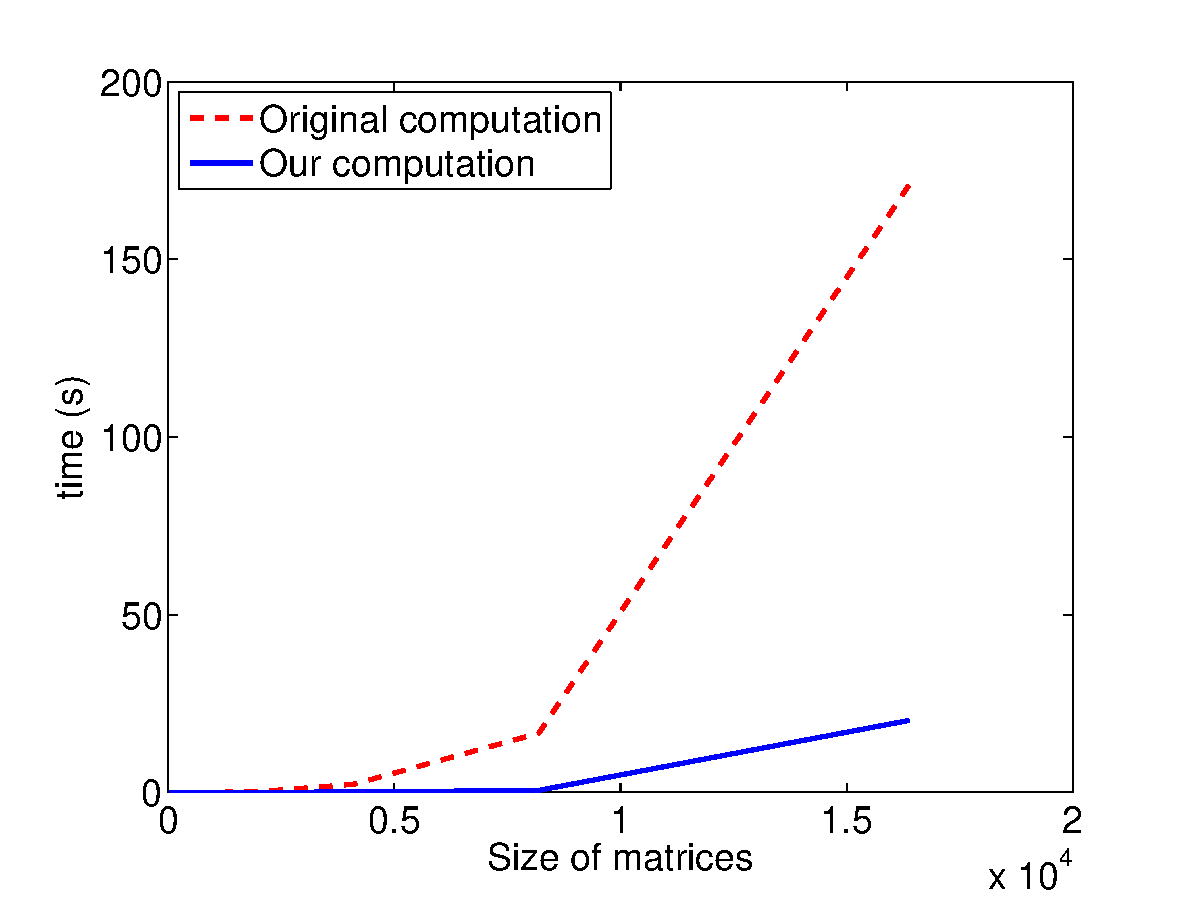
\includegraphics[width=0.55\linewidth]{img/ab.eps}
      \label{ab}
  }\quad
\subfigure[Approximations of $e^x$ using Taylor series.]{
  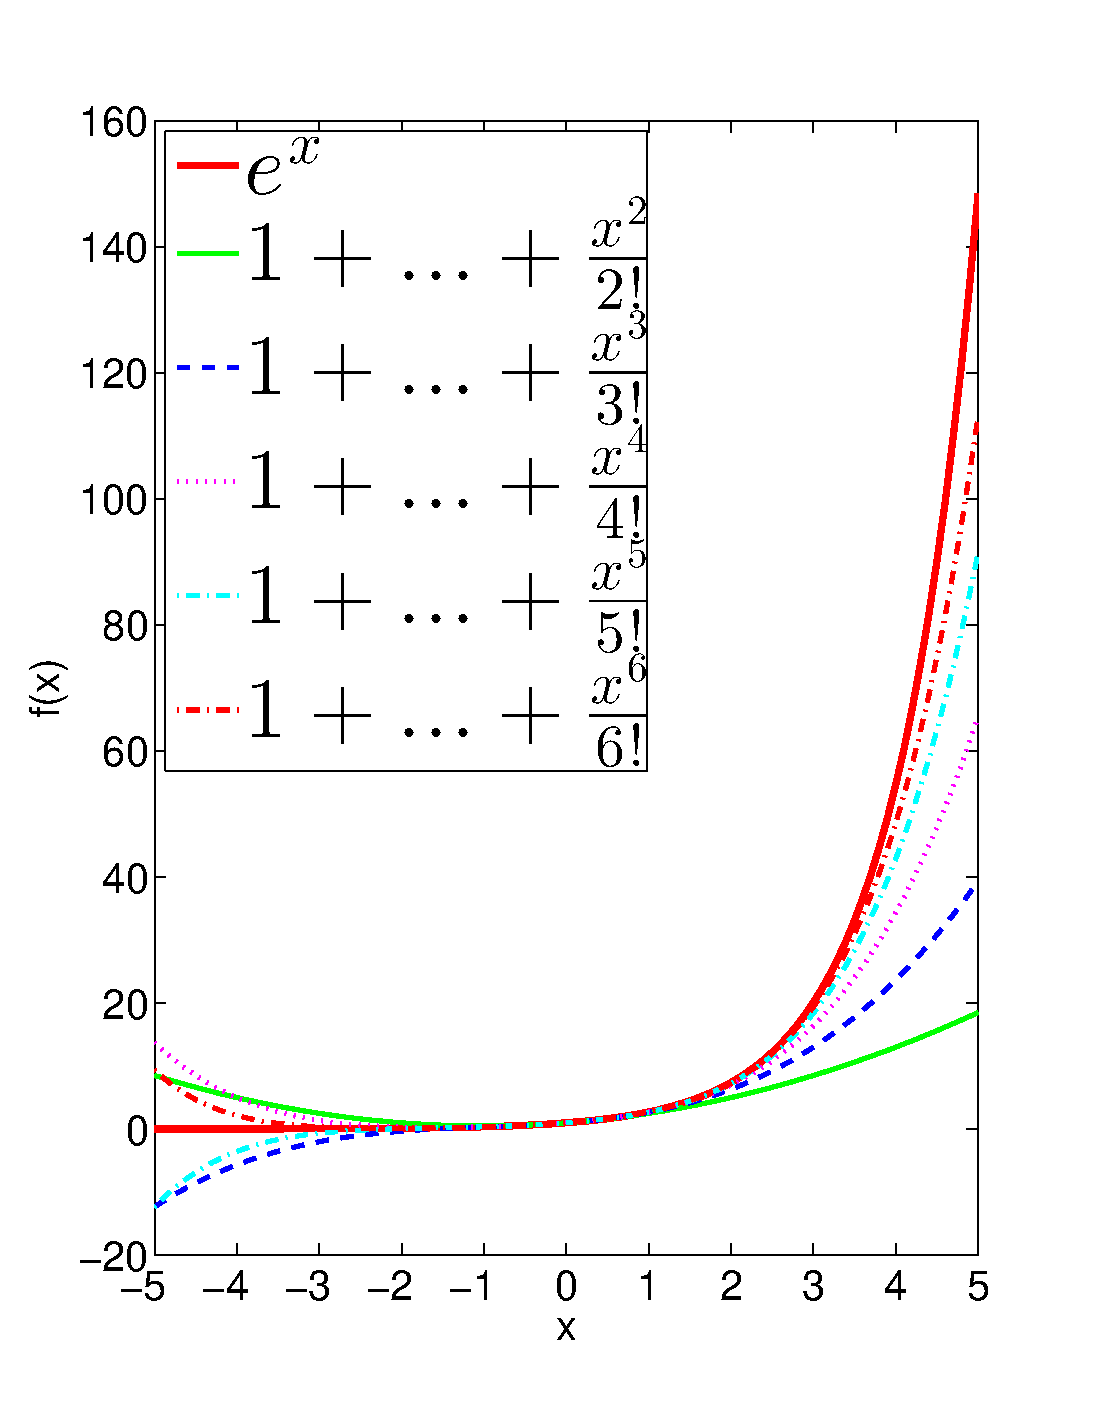
\includegraphics[width=0.32\linewidth]{img/approximations.eps} 
  \label{approximations}
  }
}

\subfigure[Comparison of computation time for naive exponential time algorithm vs our optimized derivation.]{
  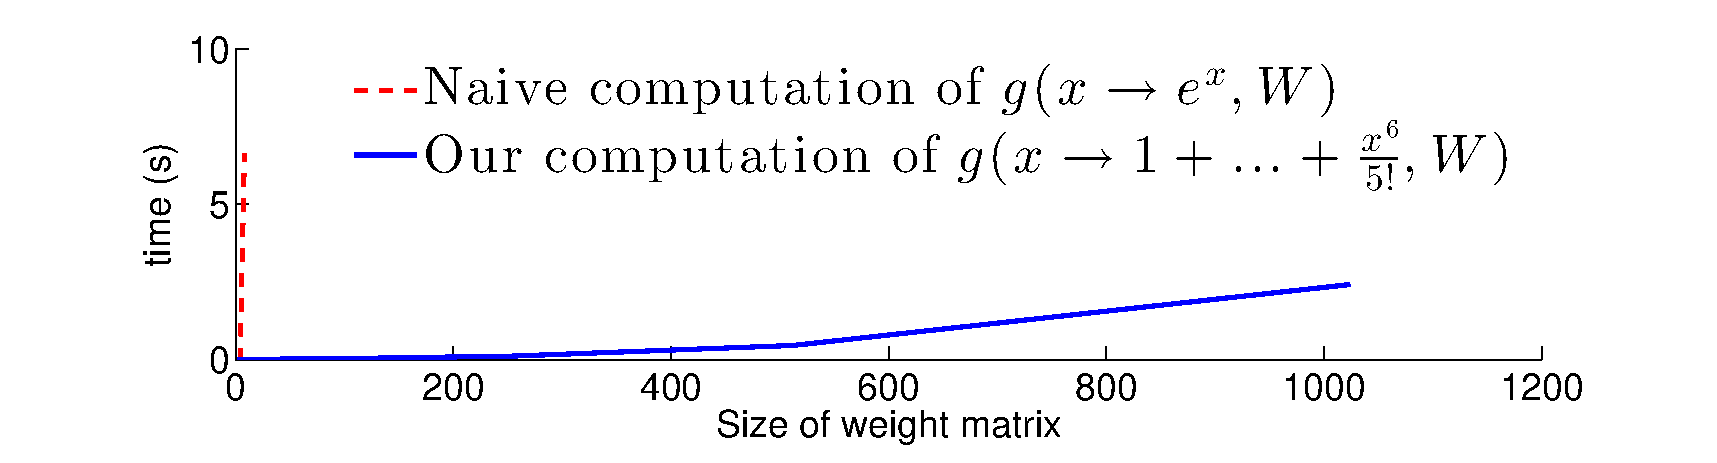
\includegraphics[scale=0.24]{img/time_approx.eps}
  \label{time_approx}
}
\vspace{-7mm}
\end{figure}

